\subsection{理论依据}
    \begin{equation*}
        span\{Cov(E(X|Y))\}\subseteq S_{Y|X}
    \end{equation*}
    将区间$(-\infty,+\infty)$划分为$k$个区间$I_i, i=1,\dots,k$,定义$\widetilde{Y}=\sum_{i=1}^kiI\{Y\in I_i\}$,则有
    \begin{equation*}
        span\{Cov(E(X|\widetilde{Y}))\}\subseteq S_{Y|X}
    \end{equation*}
\subsection{样本计算流程}
    \begin{enumerate}
        \item 将$X_1,\dots,X_n$标准化为$Z_1,\dots,Z_n$
        \item 将$[a,b]=[min{Y_i}_{i=1}^n,max{Y_i}_{i=1}^n]$划分为$k$个区间,得到$\widetilde{Y}_i$;由此计算$\bar{\mu}_i=\frac{1}{\#\{I_i\}}\sum_{Y_j\in I_i}Z_j$
        \item 计算协方差矩阵估计量$$\widetilde{M}=\sum_{i=1}^kE_n[I(Y\in I_i)] E_n(Z|\widetilde{Y}=i) E_n(Z|\widetilde{Y}=i)^T=\sum_{i=1}^k\frac{\#\{I_i\}}{n}\bar{\mu_i}\bar{\mu_i}^T$$
        \item 计算$\widetilde{M}$的前q个特征向量$u_1,\dots,u_n$,则对$S_{Y|X}$中向量的估计为$v_k=\hat{\Sigma}_{X}^{-1/2}u_k,k=1,\dots,q$
    \end{enumerate}

\subsection{确定估计后降维维度}
    设定样本量为1000,样本$X$维度为$10$,降维后维度为$2$.\\
    根据岭比率阈值准则$\hat{q} = arg\max\left\{i|\frac{\hat{\lambda_{i+1}+C_n}}{\hat{\lambda_i}+C_n}\tau\right\}$估计得到的降维后维度为1,其中设置$C_n = \frac{1}{n^\frac{1}{3} }$.

\subsection{线性函数关系}
设置降维维度为二维,即按$y=\beta_1^Tx+\beta_2^Tx+\varepsilon$,生成样本y。其中$\beta_1$是参数矩阵$\beta$的第一列向量,同理$\beta_2$,而$\varepsilon$服从均值为0,方差0.1的正态分布。得到的结果如下图所示
\begin{figure}[H]
    \centering
    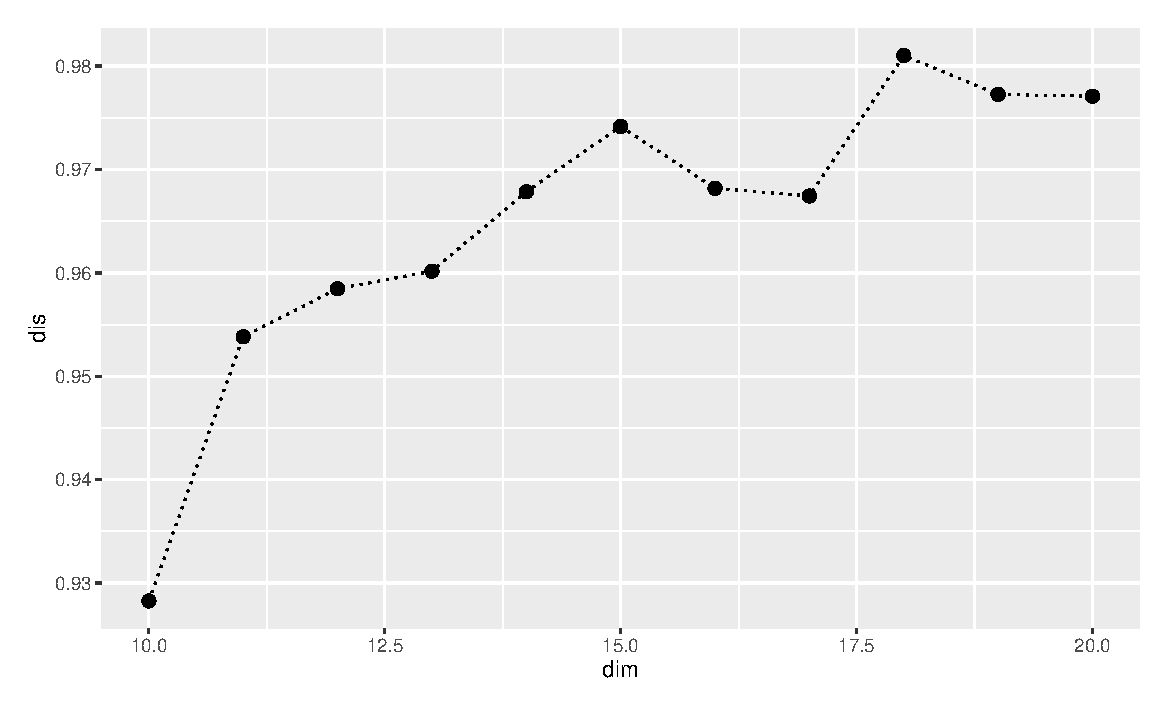
\includegraphics[width=0.8\textwidth]{image/norm_sir.eps}
    \caption{线性函数关系}
\end{figure}


\subsection{生成sin函数关系}

首先设置降维维度为二维,即按$y=\sin(2\beta_1^Tx)+\sin(\beta_2^Tx)+\varepsilon$,生成样本y。其中$\beta_1$是参数矩阵$\beta$的第一列向量,同理$\beta_2$,而$\varepsilon$服从均值为0,方差0.1的正态分布。得到的结果如下图所示
    \begin{figure}[H]
        \centering
        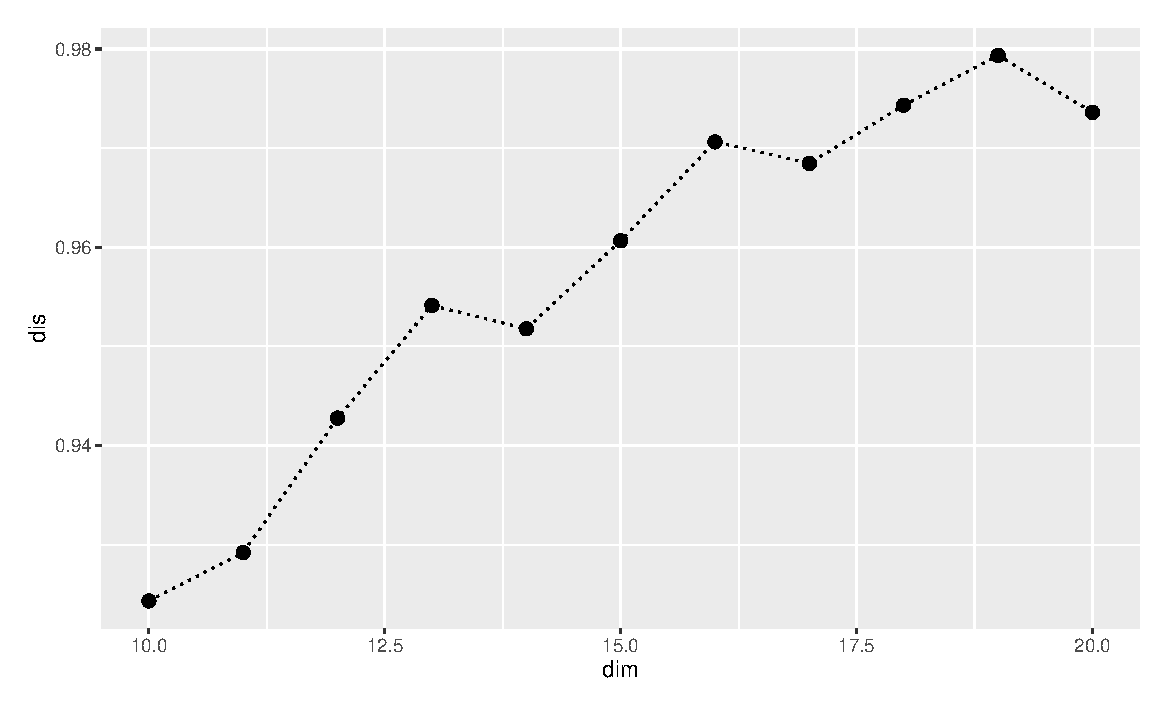
\includegraphics[width=0.8\textwidth]{image/sin_sir.eps}
        \caption{sin函数生成的数据下维度对降维效果的影响(二维)}
    \end{figure}

而降维结果为一维时,即按$y=\sin(2\beta_1^Tx)+\varepsilon$,生成样本y。与cos函数生成的数据结果比较如图所示
\begin{figure}[H]
    \centering
    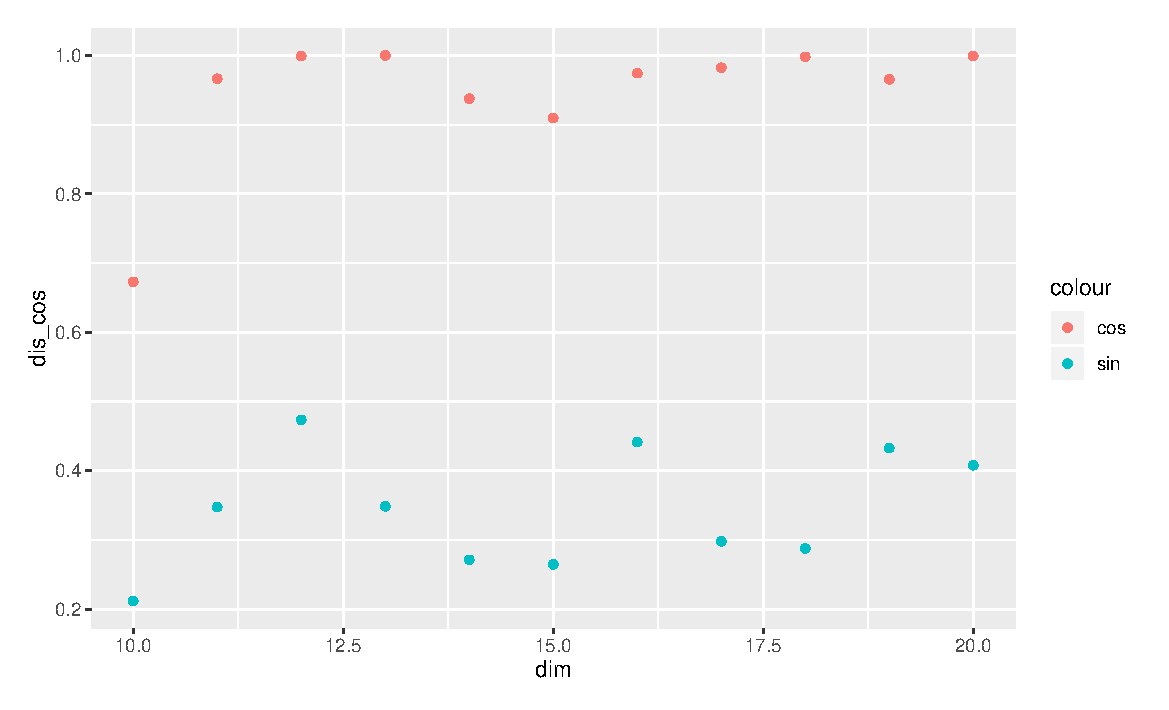
\includegraphics[width=0.8\textwidth]{image/compare_sir.eps}
    \caption{sin函数生成的数据下维度对降维效果的影响(一维)}
\end{figure}
可以看出SIR对奇函数的降维效果相较于偶函数有比较不错的改进.